\section{Interval Scheduling}

We begin by considering the interval scheduling problem. The same problem is referred to as the activity selection problem in CLRS.

Consider a set $S = \{a_1,a_2,\ldots,a_n\}$ of jobs/activities, each with a start time $s_i$ and finish time $f_i$. Two jobs are said to be compatible if they don't overlap. More formally, given activities $a_i$ and $a_j$, they are compatible if $[s_i,f_i) \cap [s_j,f_j) = \emptyset$. That is, if $s_i \geq f_j$ or $s_j \geq f_i$. The goal of the interval scheduling problem is to find a maximum-size subset of mutually compatible jobs.

Let us consider the greedy strategy for solving the interval scheduling problem. Intuitive, the globally optimal solution should leave resources/time open for as many other jobs as possible. This requires us to consider the jobs in some ``natural'' order:

\begin{itemize}
    \item Earliest start time: consider jobs in ascending order of $s_i$
    \item Earliest finish time: consider jobs in ascending order of $f_i$
    \item Shortest inverval: consider jobs in ascending order of $f_i - s_i$ 
    \item Fewest conflicts: for each job $a_i$, count the remaining number of conflicting jobs $c_i$ and schedule in ascending order of $c_i$. 
\end{itemize}

Not all of those strategies work. Here are some counterexamples (Figure \ref{fig:greedy-interval-scheduling-counterexample}).

\begin{figure}[htbp]
    \centering
    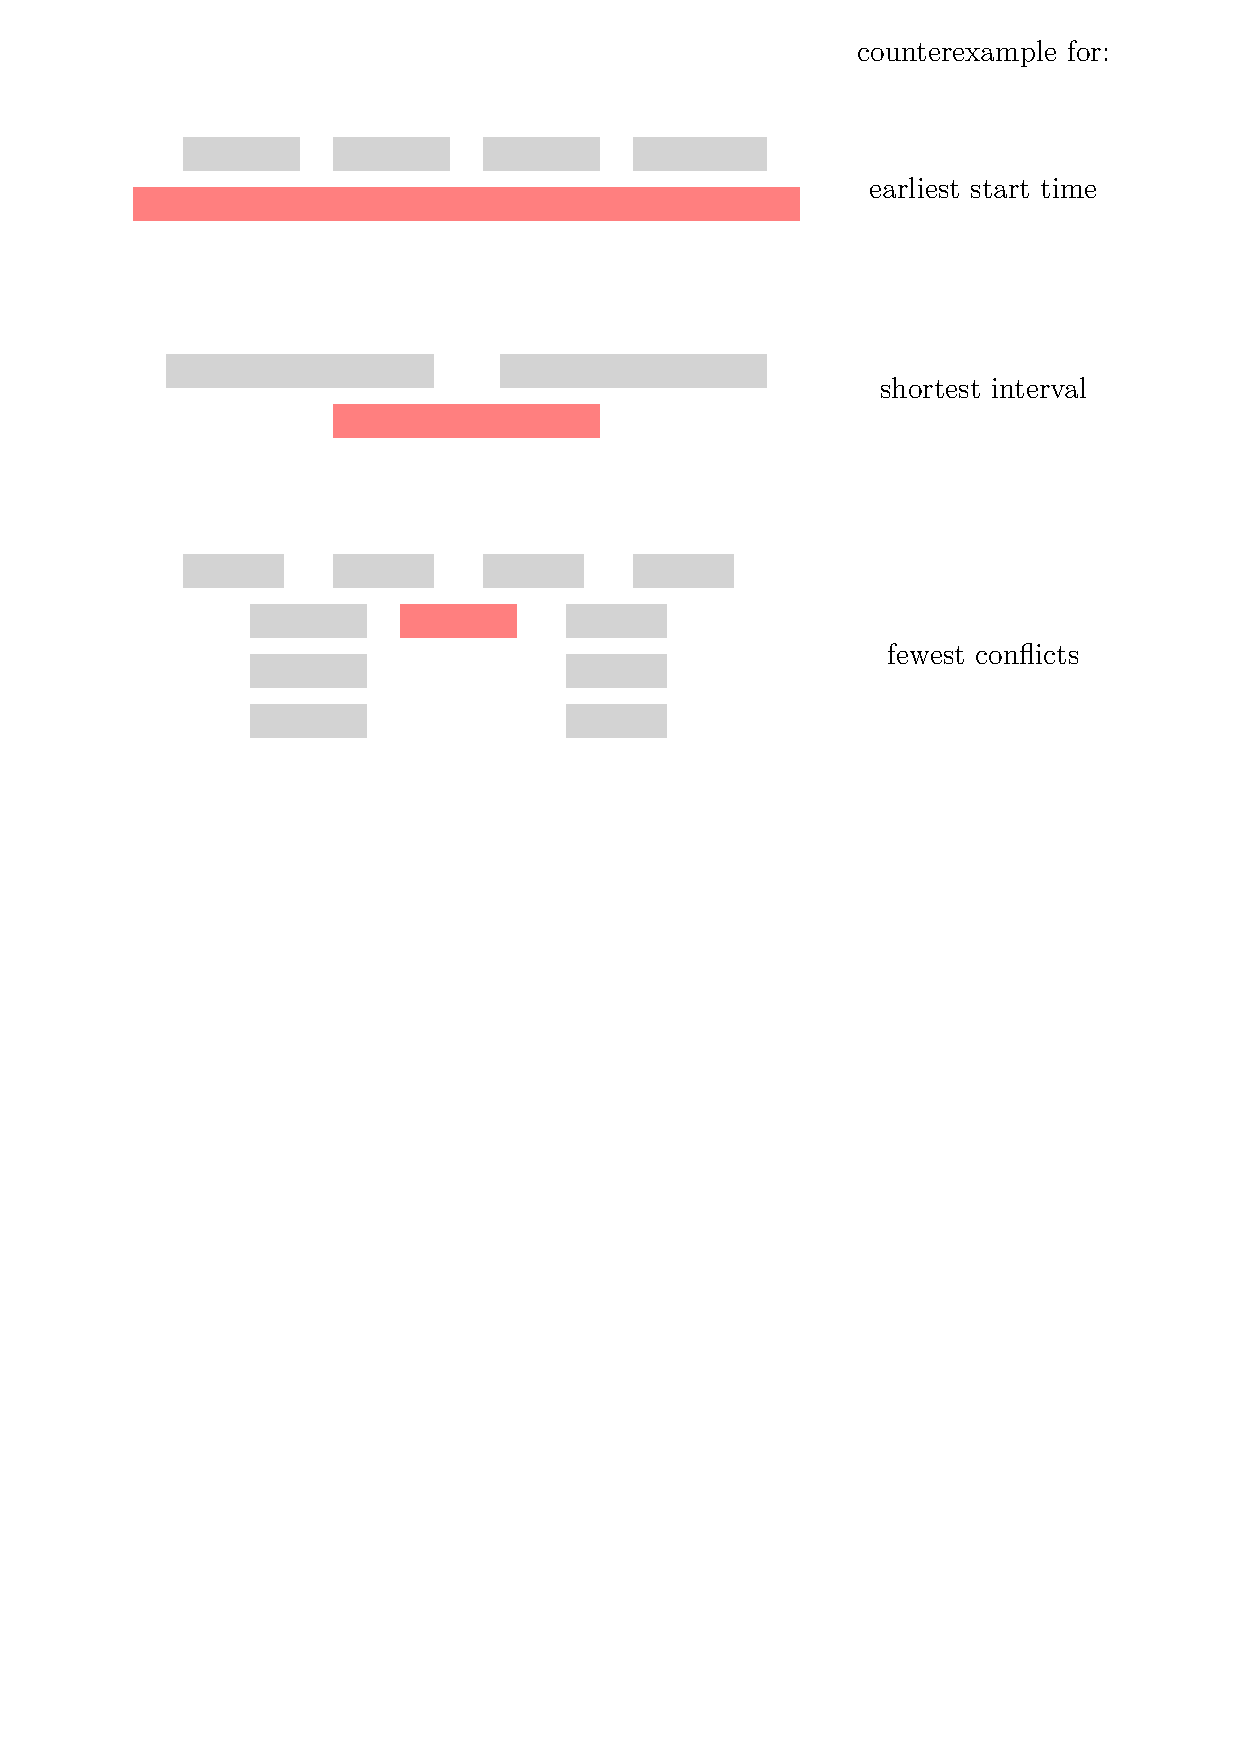
\includegraphics[width=0.7\linewidth]{greedy/interval-scheduling-counterexample.pdf}

    \hfill

    \caption{Counterexamples for the greedy strategies that do not work for the interval scheduling problem. The interval that satisfies the greedy strategy but leads to incorrect global solution is highlighted in red.}
    \label{fig:greedy-interval-scheduling-counterexample}
\end{figure}

Therefore, we choose earliest finish time as our greedy strategy, which we can implement into this recursive algorithm

\begin{codebox}
    \Procname{$\proc{Interval-Scheduling-Recursive}(S,k,n)$}
    \li $m = k + 1$
    \li \While $m \leq n$ and $S[m].s < S[k].f$ \Do
        \li $m = m + 1$
    \End
    \li \If $m \leq n$ \Then
        \li \Return $\{S[m]\} \cup \proc{Interval-Scheduling-Recursive}(S,m,n)$
    \li \Else
        \li \Return $\emptyset$ 
\end{codebox}

As a precondition, we assume that the array of jobs $S$ is sorted in monotonically increasing order by finish time. $S[i].s$ denotes the starting time of the $i$th job, and $S[i].f$ denotes the finish time of the $i$th job. $k$ is the job being considered. In each call to the recursive algorithm, we starts from $m = k+1$ and increment $m$ until we find a job with starting time $S[m].s$ strictly lower than the finish time of $S[k]$. This is the job that is selected by our greedy strategy in the current recursive call. After finding this $m$, we return the union of $\{S[m] = a_m\}$ and the maximum-size subset of $S_m$ returned by the recursive call $\proc{Interval-Scheduling-Recursive}(S,m,n)$.

The initial call that solves the problem globally is $\proc{Interval-Scheduling-Recursive}(S,0,n)$ where $n$ is the number of jobs to be considered.

This algorithm can be easily converted into an iterative algorithm.

\begin{codebox}
    \Procname{$\proc{Interval-Scheduling}(S)$}
    \li $n = \attrib{S}{length}$ 
    \li $S' = \{a_1\}$
    \li $k = 1$
    \li \For $m = 2$ to $n$ \Do
        \li \If $S[m].s \geq S[k].f$ \Then
            \li $S' = S' \cup \{S[m]\}$
            \li $k = m$
        \End
    \End
    \li \Return $S'$ 
\end{codebox}

Sorting the array of jobs takes $O(n \log n)$ time, and going over the sorted the list and check each job's compatibility takes $O(n)$ in total.

\section{Proving Optimality}

As we have demonstrated earlier in Figure \ref{fig:greedy-interval-scheduling-counterexample}, greedy strategy does not always work. It is important for us to ensure (prove) that the locally optimal greedy choice leads to a globally optimal solution. Here, we will present three equally valid proofs for the optimality of the greedy algorithm for the interval scheduling problem.

\begin{theorem}
    The greedy algorithm using earliest finish time is optimal. More formally, the algorithm returns a maximum-size set of disjoint jobs $\{a_1,\ldots,a_m\} \subseteq S$
\end{theorem}

\begin{proof}[Proof (by contradiction)]
    Suppose, for contradiction, that the greedy algorithm using earlies finish time is not optimal. Let $i_1,i_2,\ldots,i_k$ be the sequence of jobs selected by the algorithm, and let $j_1,j_2,\ldots,j_m$ be the correct solution where $m>k$. Let $r$ be the largest possible value such that $i_{r+1} \neq j_{r+1}$. That is, the $(r+1)$th job is the first job where the two sequences begin to differ. 

    Both $i_{r+1}$ and $j_{r+1}$ must be compatible with previous choices of $i$ and $j$, respectively. Let $i_1=j_1,i_2=j_2,\ldots,i_r=j_r,i_{r+1},j_{r+2}, \ldots, j_m$ be a new sequence of jobs. This is the optimal solution with $j_{r+1}$ replaced with $i_{r+1}$. By assumption, the greedy solution is not optimal so $j_{r+1}$ is not selected by the greedy algorithm and thus $i_{r+1} \leq j_{r+1}$. So, the new sequence of jobs is still feasible because $i_{r+1} \leq j_{r+1}$. The algorithm is still optimal because all $m$ disjoint jobs are scheduled. But then, $i_{r+1}$ is not different from $j_{r+1}$, which implies that $r$ is not the maximum value such that $i_{r+1} \neq j_{r+1}$. This is a contradiction. Therefore, the greedy algorithm is optimal.
\end{proof}

\begin{proof}[Proof (by induction)]
    Let $S_k$ be the subset of jobs selected by the greedy algorithm after considering the first $k$ jobs in increasing order of finish time. We say that $S_k \subseteq S$ is promising if it can be extended to the optimal solution ($S_k$ is part of the optimal solution). More formally, $S_k$ is promising if there exists $T \subseteq \{ a_{k+1},\, \ldots,\, a_{n}\}$ such that $O_k = S_k \cup T$ is optimal.

    We want to show that for all $k \in \{0,1,\ldots,n\}$, $S_k$ is promising.

    \textbf{Base case}: When $k=0$, $S_0=\emptyset$. The claim is vacuously true.
    
    \textbf{Inductive step}: Let $j \in \N$ be arbitrary. Suppose that the claim holds for $k = j - 1$ and that $S_{j-1}$ is promising. For $S_j$, there are two possibilities:

    (1) The greedy algorithm did not select job $a_j$ (i.e. $s_{j+1} < f_j$), so $S_j = S_{j-1}$. This implies that $a_j$ is not compatible with some job in $S_{j-1}$. Since $S_{j-1} \subseteq O_{j-1}$, $O_{j-1}$ does not include $a_j$. $O_j = O_{j-1}$ does not include $a_j$, so $S_j$ can be extended to $O_j$ and $S_j$ is promising.
    
    (2) The greedy algorithm selected job $a_j$ (i.e. $s_{j+1} \geq f_j$), so $S_j = S_{j-1} \cup \{a_j\}$. Consider the earliest job $a_r$ in $O_{j-1} - S_{j-1}$. Consider $O_j = O_{j-1} - \{a_r\} \cup \{a_j\}$. $O_j$ is still feasible since jobs in $O_{j-1}$ are disjoint, $a_r$ is the first to finish, and the finish time of $a_j$ is earlier or equal to the finish time of $a_r$. Hence, $S_j$ can be extended to $O_j$.

    \begin{center}
        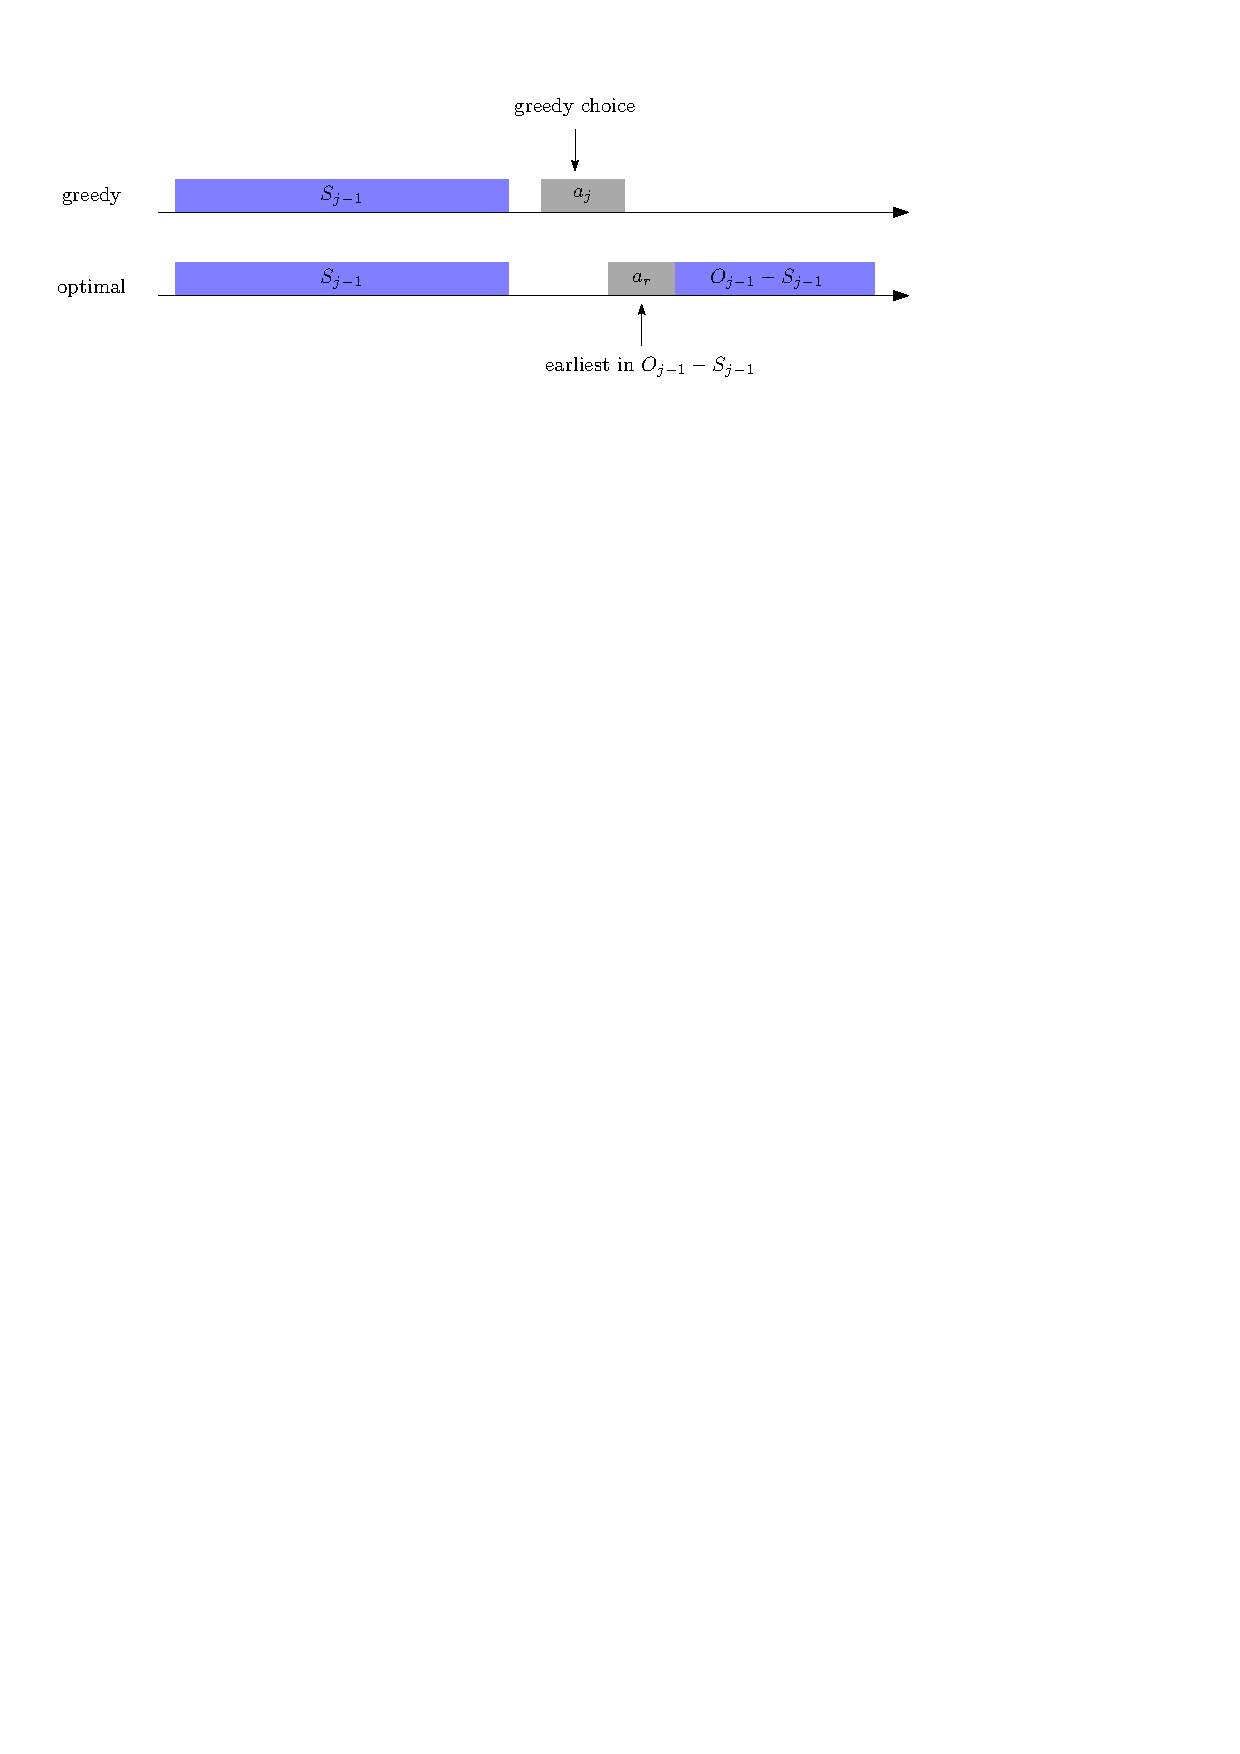
\includegraphics[width=0.7\linewidth]{greedy/interval-scheduling-optimality-proof.pdf}
    \end{center}
    By induction, the claim is true for all $k \in \{0,1,\ldots,n\}$.
\end{proof}

The previous two proofs use the technique known as the exchange argument. They both rely on the argument that if the greedy solution after $j$ iterations can be extended to an optimal solution, then the greedy solution after $j+1$ iterations can also be extended to an optimal solution by exchanging some interval with one chosen based on the greedy strategy. 

The last proof uses what we call an ``\textit{\textbf{charging argument}}''. In this case, the charging argument charges each interval of an optimal solution (or arbitrary solution) to a unique interval in the greedy solution. Charging arguments are also used in approximation algorithms (for example, to prove that an algorithm is a $k$-approximation).

\begin{proof}[Proof (by charging argument)] \index{charging argument}
    Given a set of jobs $S = \{a_1,\ldots,a_n\}$, let $O$ be an optimal solution of the interval scheduling problem. Let $S'$ be the solution given by the greedy algorithm using earliest finish time. We want to find a one-to-one function $h:\, O \to S'$. For any job $j \in O$, define $h(j)$ as the interval $j' \in S'$ that intersects $j$ and has the earliest finish time amongst intervals in $S'$ intersecting $j$.

    We claim that the $h$ is well-defined so $h(j)$ must exists for all $j$. This is proved by contradiction. Suppose, for contradiction, that there exists a $j \in O$ where $h(j)$ as we defined does not exist. By definition, this means no interval in $S'$ intersects with $j$. This implies that $j$ is compatible with every interval in $S'$, so the greedy strategy would have selected $j$ and $j$ would be part of $S'$. But then if $j \in S'$, $j$ intersects with itself. This is a contradiction. $h(j)$ \textbf{exists} for all $j \in O$. Furthermore, $h(j)$ is \textbf{unique} because all intervals in $S'$ are mutually disjoint, and every interval in $S'$ that intersects $j$ have distinct finish time.

    We then show that $h$ is \textbf{injective}, similarly by contradiction. Assume that there are two intervals $j_1,j_2 \in O$ such that $h(j_1) = h(j_2) = j' \in S'$. Without loss of generality, suppose that the finish time of $j_1$ is earlier than $j_2$. $j_1$ and $j_2$ are disjoint because they are both in $O$, which implies that $f_1 \leq s_2 < f_2$. Since $j' \in S'$, the greedy algorithm must have encountered $j'$ before $j_1$ and $j_2$. Thus, $f' \leq f_1$. But then, this implies that $f' \leq f_1 \leq s_2 < f_2$. That is, $j'$ and $j_2$ do not overlap. This is a contradiction because if they do not intersect, $h(j_2) \neq j'$. Therefore, $h$ is injective.
    
    Since there exists an one-to-one function $h:\; O \to S'$, by the charging argument, the greedy algorithm for the interval scheduling problem is optimal.
\end{proof}

More generally, we have shown that $|O| \leq |S'|$, which implies the optimality of the algorithm (that the algorithm returns the maximum-size subset).

\section{Interval Coloring (Interval Partition)}

Let us know consider a modified version of the original interval scheduling problem. Suppose that we are given a set of intervals. We want to color all intervals so that intervals with the same color do not intersect while using the minimum number of colors. This problem is also known as the interval partitioning problem.

Similar to interval scheduling, let's take a look at the few possible choices for our greedy strategy:
\begin{itemize}
    \item Earliest start time
    \item Earliest finish time
    \item Shortest interval
    \item Fewest conflicts
\end{itemize}
We can show using counterexamples that the last three heuristics, earliest finish time, shortest interval, and fewest conflicts, do not work. We will prove that the earliest start time greedy choice gives us a globally optimal solution for the interval partitioning problem.

The proof for this is somewhat similar to the charging argument that we used to prove the optimality of interval scheduling. We attempt to bound the size of the solution set in order to show that it is optimal (miminal). In the charging argument, we bound the size by showing that there exists an one-to-one function. In this proof, we will skip that part and instead bound the size directly.

\begin{lemma} \label{lem:interval-partition-upper-bound}
    Given a set of intervals, let $d$ be the maximum number of intersecting intervals at any time. The number of partitions (colors) given by any algorithms that solve the interval partitioning problem must be at least $d$.
\end{lemma}

\begin{proof}
    By contradiction.
\end{proof}

\begin{lemma} \label{lem:interval-partition-lower-bound}
    Let $d$ be defined as in the previous lemma. The greedy algorithm using earliest start time produces a solution with at most $d$ partitions.
\end{lemma}

\begin{proof}
    Let $d'$ be the number of partitions produced by the greedy algorithm. Suppose for contradiction that the algorithm used more than $d$ partitions. Consider the first time that the greedy algorithm used $d+1$ partitions. Suppose this happens when the algorithm is trying to assign a partition to the interval $j$. This implies that there are $d$ intervals intersecting $j$. Let $s_j$ be the starting time of $j$. These $d$ intervals must contain $s_j$. This is because all the previous $d$ intervals have starting time earlier than $s_j$. So it must be that case that $s_j$ is after or at the starting time of the other $d$ intervals. But then, this implies that there are $d+1$ overlapping intervals at $s_j$, contradicting the fact that there are at most $d$ intersecting intervals at any time.
\end{proof}

\begin{corollary}
    The greedy algorithm produces a solution with exactly $d$ partitions.
\end{corollary}

\begin{proof}
    Follows immediately from the Lemma \ref{lem:interval-partition-upper-bound} and \ref{lem:interval-partition-lower-bound}.
\end{proof}

Hence the theorem:

\begin{theorem}
    The greedy algorithm using earliest starting time as greedy choice is optimal.
\end{theorem}

This greedy algorithm is implemented as follows. Suppose, as a precondition, that $S$ is sorted in increasing order of starting time, and that elements in $Q$ contains objects of $\proc{Interval}$s that are indexed by finish time.

\begin{codebox}
    \Procname{$\proc{Interval-Partitioning}(S)$}
    \li $d = 0$
    \zi \Comment{initialize PQ using finish time as key} 
    \li $Q = \proc{Priority-Queue}(\id{key}=f)$ 
    \li \For $i = 1$ \textbf{to} $\attrib{S}{length}$ \Do
        \li $k = \proc{Extract-Min}(Q)$
        \li \If $k \isequal \const{nil}$ \Then
            \li $d = d + 1$
            \li $\id{interval} = $ \textbf{new} $\proc{Interval}(i.f)$ 
            \li $\proc{Insert}(Q,\id{interval})$
        \End
        \li \If $i.s > \proc{Min}(Q)$ \Then
            \zi \Comment{if $i$ is compatible with $k$, allocate $i$ to $k$}
            \li $k.f = i.f$
            \li $\proc{Insert}(Q, k)$
        \li \Else
            \zi \Comment{otherwise, create new classroom $d+1$}
            \li $d = d + 1$
            \li $\proc{Insert}(Q, k)$
            \li $\id{interval} = $ \textbf{new} $\proc{Interval}(i.f)$
            \li $\proc{Insert}(Q,\id{interval})$
        \End
    \End
    \li \Return $d$
\end{codebox}

This algorithm runs in $O(n \log n)$ time. This is the case regardless of whether or not we consider sorting as part of the algorithm because the $n$ priority queue operation is going to cost $O(n \log n)$ anyway, assuming the priority is implemented as a min-heap.

\section{Greedy Strategy}

The greedy strategy can be generalized as follows:

\begin{enumerate}
    \item Cast the optimization problem as one in which we make a choice and are left with one subproblem to solve.
    \item Prove that there is always an optimal solution to the original problem that makes the greedy choice, so that the greedy choice is always safe.
    \item Demonstrate optimal substructure by showing (typically by contradiction or induction) that, having made the greedy choice, what remains is a subproblem with the property that if we combine an optimal solution to the subproblem with the greedy choice we have made, we arrive at an optimal solution to the original problem.
\end{enumerate}

\index{greedy property}
The important property that requires us to prove when implementing a greedy algorithm is the \textit{\textbf{greedy property}}. It tells us that we can assemble a globally optimal solution from locally optimal choices. The exchange argument for the proof (the first two proofs that we have seen for interval scheduling) argues that we can modify the globally optimal solution to substitute the greedy choice for some other choice, resulting in one similar, but smaller, subproblem.